% --- chapter
\newcommand{\chapter}[2][]{
	\newcommand{\chapname}{#2}
	\begin{flushleft}
		\begin{minipage}[t]{\linewidth}
			
\includegraphics[height=1cm]{hdht-logo.png}
			\hspace{0pt}	
			\sffamily\bfseries\large Bài  36. Năng lượng liên kết của hạt nhân. Phản ứng hạt nhân
			\begin{flushleft}
				\huge\bfseries #1
			\end{flushleft}
		\end{minipage}
	\end{flushleft}
	\vspace{1cm}
	\normalfont\normalsize
}
%-----------------------------------------------------
\chapter[Các định luật bảo toàn\\ trong phản ứng hạt nhân]{Các định luật bảo toàn trong phản ứng hạt nhân}
\section{Lý thuyết}

\subsection{Các định luật bảo toàn trong phản ứng hạt nhân}
	Xét phản ứng hạt nhân
	\begin{equation}
	^{A_1}_{Z_1}A + ^{A_2}_{Z_2}B \rightarrow ^{A_3}_{Z_3}C + ^{A_4}_{Z_4}D
	\end{equation}
	\subsubsection{Định luật bảo toàn điện tích}
	Trong phản ứng hạt nhân, tổng đại số điện tích các hạt tương tác bằng tổng đại số điện tích các hạt sản phẩm
	\begin{equation}
	Z_1+Z_2=Z_3+Z_4.
	\end{equation}
	\subsubsection{Định luật bảo toàn số khối}
	Trong phản ứng hạt nhân, tổng số nuclon các hạt tương tác bằng tổng số nuclon các hạt sản phẩm
	\begin{equation}
	A_1+A_2=A_3+A_4.
	\end{equation}
	
	\subsubsection{Định luật bảo toàn năng lượng toàn phần}
	Năng lượng toàn phần bao gồm động năng và năng lượng nghỉ. Trong phản ứng hạt nhân, tổng năng lượng toàn phần của các hạt bằng tổng năng lượng toàn phần của các hạt sản phẩm
	\begin{equation}
	E_A+E_B=E_C+E_D
	\end{equation}
	\begin{equation}
	\Leftrightarrow m_Ac^2+ W_{\textrm{đ }A} + m_Bc^2+W_{\textrm{đ }B} = m_Cc^2+ W_{\textrm{đ }C} + m_Dc^2+W_{\textrm{đ }D}
	\end{equation}
	\begin{equation}
	\Leftrightarrow W_\textrm{đ trước} + (m_A+m_B)c^2 = W_\textrm{đ sau} + (m_C+m_D)c^2 .
	\end{equation}
	
	\subsubsection{Định luật bảo toàn động lượng}
	Trong phản ứng hạt nhân, vectơ tổng động lượng của các hạt tương tác bằng vectơ tổng động lượng của các hạt sản phẩm.
	\begin{equation}
	\vec{p}_A + \vec{p}_B = \vec{p}_C + \vec{p}_D
	\end{equation}
	\begin{equation}
	\Leftrightarrow m_A\vec{v}_A + m_B\vec{v}_B = m_C\vec{v}_C + m_D\vec{v}_D.
	\end{equation}

\subsection{Năng lượng tỏa ra hay thu vào trong phản ứng hạt nhân}
	Do tính chất không bảo toàn khối lượng nghỉ, nhưng lại bảo toàn năng lượng toàn phần của hệ trong phản ứng hạt nhân, nên các phản ứng hạt nhân có thể tỏa ra năng lượng hoặc thu vào năng lượng. 
	
	Gọi $m_\text{trước}$ là tổng khối lượng nghỉ của các hạt trước phản ứng và $m_\text{sau}$ là tổng khối lượng nghỉ của các hạt sau phản ứng. Năng lượng của một phản ứng hạt nhân là
	\begin{equation}
	\Delta W = \left(m_\text{trước} - m_\text{sau}\right) c^2;
	\end{equation}
	trong đó:
	\begin{itemize}
		\item Nếu $m_\text{trước}$ > $m_\text{sau} \Rightarrow \Delta W >0$ thì phản ứng tỏa năng lượng;
		\item Nếu $m_\text{trước}$ < $m_\text{sau} \Rightarrow \Delta W < 0$ thì phản ứng thu năng lượng.
	\end{itemize}
	
%	\manatip{\textbf{Dư tỏa nợ thu} (Dương tỏa âm thu - Ngược lại với cân bằng hóa học).}
	
\section{Mục tiêu bài học - Ví dụ minh họa}

	\begin{dang}{Năng lượng phản ứng, nhiên liệu cần đốt.}
	
		\ppgiai{
		
		Xét phản ứng hạt nhân
		\begin{equation*}
		^{A_1}_{Z_1}A + ^{A_2}_{Z_2}B \rightarrow ^{A_3}_{Z_3}C + ^{A_4}_{Z_4}D
		\end{equation*}
		
		Năng lượng của phản ứng hạt nhân có thể tính theo các công thức sau:
		\begin{itemize}
			\item Tính theo khối lượng
			\begin{equation*}
			\Delta W = \left(m_\text{trước} - m_\text{sau}\right) c^2;
			\end{equation*}
			\begin{equation*}
			\Leftrightarrow \Delta W = \left[ \left(m_A + m_B\right)  - \left( m_C + m_D\right)\right]  c^2;
			\end{equation*}
			trong đó: $m_A$, $m_B$, $m_C$, $m_D$ lần lượt là khối lượng nghỉ của các hạt nhân $X_A$, $X_B$, $X_C$, $X_D$.
			
			\item Tính theo độ hụt khối
			\begin{equation*}
			\Delta W = \left(\Delta m_\text{sau} - \Delta m_\text{trước}\right) c^2;
			\end{equation*}
			\begin{equation*}
			\Leftrightarrow \Delta W = \left[\left(\Delta m_C + \Delta m_D \right) -  \left(\Delta m_A + \Delta m_B\right)\right] c^2;
			\end{equation*}
			trong đó: $\Delta m_A$, $\Delta m_B$, $\Delta m_C$, $\Delta m_D$ lần lượt là độ hụt khối của các hạt nhân $X_A$, $X_B$, $X_C$, $X_D$.
			
			\item Tính theo năng lượng liên kết, năng lượng liên kết riêng
			\begin{equation*}
			\Delta W = \left(W_\text{lk sau} - W_\text{lk trước}\right) c^2;
			\end{equation*}
			\begin{equation*}
			\Leftrightarrow \Delta W = \left[\left(W_{\textrm{lk }C} + W_{\textrm{lk }D} \right) -  \left(W_{\textrm{lk }A} + W_{\textrm{lk }B}\right)\right] c^2;
			\end{equation*}
			\begin{equation*}
			\Leftrightarrow \Delta W = \left[\left(A_C\cdot W_{\textrm{lkr }C} + A_D\cdot W_{\textrm{lkr }D} \right) -  \left(A_A\cdot W_{\textrm{lkr }A} + A_B\cdot W_{\textrm{lkr }B}\right)\right] c^2;
			\end{equation*}
			trong đó:
			\begin{itemize}
			\item $W_{\textrm{lk }A}$, $W_{\textrm{lk }B}$, $W_{\textrm{lk }C}$, $W_{\textrm{lk }D}$ lần lượt là năng lượng liên kết của các hạt nhân $X_A$, $X_B$, $X_C$, $X_D$.
			
			\item $W_{\textrm{lkr }A}$, $W_{\textrm{lkr }B}$, $W_{\textrm{lkr }C}$, $W_{\textrm{lkr }D}$ lần lượt là năng lượng liên kết riêng của các hạt nhân $X_A$, $X_B$, $X_C$, $X_D$.
			
			\item $A_A$, $A_B$, $A_C$, $A_D$ lần lượt là số khối của các hạt nhân $X_A$, $X_B$, $X_C$, $X_D$.
			\end{itemize}
				
			\item Tính theo động năng
			\begin{equation*}
			\Delta W = \left(W_\textrm{đ sau} - W_\textrm{đ trước}\right) c^2;
			\end{equation*}
			\begin{equation*}
			\Leftrightarrow \Delta W = \left[ \left(W_{\textrm{đ }C} + W_{\textrm{đ }D}\right)  - \left( W_{\textrm{đ }A} + W_{\textrm{đ }B}\right)\right]  c^2;
			\end{equation*}
			trong đó: $W_{\textrm{đ }A}$, $W_{\textrm{đ }B}$, $W_{\textrm{đ }C}$, $W_{\textrm{đ }D}$ lần lượt là động năng của các hạt nhân $X_A$, $X_B$, $X_C$, $X_D$.
		\end{itemize}}
		
		\luuy{
			Năng lượng tương ứng với khối lượng $\SI{1}{u}$ được xác định
			\begin{equation*}
			\SI{1}{\atomicmassunit}\cdot c^2=\SI{931,5}{\mega\electronvolt}.
			\end{equation*}
			}
			
		\viduii{2}
		{
		[THPT QG 2017 - Mã đề 206] Trong một phản ứng hạt nhân, tổng khối lượng nghỉ của các hạt trước phản ứng là $\SI{37,9638}{u}$ và tổng khối lượng nghỉ các hạt sau phản ứng là  $\SI{37,9656}{u}$. Lấy $\SI{1}{u}=\SI{931,5}{\mega\electronvolt/c^2}$ . Phản ứng này
		
		\begin{mcq}(2)
			\item tỏa năng lượng $\SI{1,68}{\mega\electronvolt}$.
			\item thu năng lượng $\SI{1,68}{\mega\electronvolt}$.
			\item thu năng lượng $\SI{16,8}{\mega\electronvolt}$.
			\item tỏa năng lượng $\SI{16,8}{\mega\electronvolt}$.
		\end{mcq}}
	{
		\begin{center}
			\textbf{Hướng dẫn giải}
		\end{center}
		
		Năng lượng của phản ứng hạt nhân là
			\begin{eqnarray*}
			\Delta W &=& \left(m_\text{trước} - m_\text{sau}\right) c^2 \\
			 	   	&=& \left(\SI{37,9638}{u} - \SI{37,9656}{u}\right) c^2\\
				  	&=&\left(\SI{37,9638}{} - \SI{37,9656}{}\right) \text{u}c^2\\
					 &=&\left(\SI{37,9638}{} - \SI{37,9656}{}\right) \cdot\SI{931,5}{\mega\electronvolt/c^2}\cdot c^2\\
					&=&-\SI{1,68}{\mega\electronvolt}.
			\end{eqnarray*}
		
		Vì $\Delta W = -\SI{1,68}{\mega\electronvolt} < 0$ nên phản ứng thu năng lượng $\SI{1,68}{\mega\electronvolt}$.
		
		\begin{center}
			\textbf{Câu hỏi tương tự}
		\end{center}
		
Giả sử trong một phản ứng hạt nhân, tổng khối lương hai hạt trước phản ứng lớn hơn tổng khối lượng hai hạt sau phản ứng là $\SI{0.02}{u}$. Cho $\SI{1}{u} = \SI{931.5}{MeV/c^2}$. Phản ứng hạt nhân này
	\begin{mcq}(2)
		\item tỏa năng lượng $\SI{1.863}{MeV}$.
		\item thu năng lượng $\SI{1.863}{MeV}$.
		\item tỏa năng lượng $\SI{18.63}{MeV}$.
		\item thu năng lượng $\SI{18.63}{MeV}$.
	\end{mcq}
		
		\textbf{Đáp án:} C.
		}
		\viduii{2}
		{
		[Đề thi đại học khối A năm 2009] Cho phản ứng hạt nhân $^3_1\text{T} + ^2_1 \text{D} \rightarrow ^4_2\text{He} + X$. Lấy độ hụt khối của hạt nhân $\text{T}$, hạt nhân $\text{D}$, hạt $\text{He}$ lần lượt là $\SI{0,009106}{u}$; $\SI{0,002491}{u}$; $\SI{0,030382}{u}$ và $\SI{1}{u}=\SI{931,5}{\mega\electronvolt/c^2}$. Năng lượng tỏa ra của phản ứng xấp xỉ bằng
		
		\begin{mcq}(2)
			\item $\SI{15,017}{\mega\electronvolt}$.
			\item $\SI{200,025}{\mega\electronvolt}$.
			\item $\SI{17,498}{\mega\electronvolt}$.
			\item $\SI{21,076}{\mega\electronvolt}$.
		\end{mcq}
		}
		{\begin{center}
			\textbf{Hướng dẫn giải}
		\end{center}
		
		Năng lượng của phản ứng hạt nhân là
		
		\begin{eqnarray*}
		\Delta W &=& \left(\Delta m_\text{sau} - \Delta m_\text{trước}\right) c^2 \\
		&=& \left[\left(\Delta m_\text{He} + \Delta m_\text{X} \right) -  \left(\Delta m_\text{T} + \Delta m_\text{D}\right)\right] c^2\\
		&=& \left[\left(\SI{0,030382}{u} + 0 \right) -  \left(\SI{0,009106}{u} + \SI{0,002491}{u}\right)\right] c^2\\
		&=& \left[\left(\SI{0,030382}{} \right) -  \left(\SI{0,009106}{} + \SI{0,002491}{}\right)\right] \text{u} c^2\\
		&=& \left[\SI{0,030382}{}  -  \left(\SI{0,009106}{} + \SI{0,002491}{}\right)\right] \cdot\SI{931,5}{\mega\electronvolt/c^2}\cdot c^2\\
		&=&\SI{17,498}{\mega\electronvolt}.
		\end{eqnarray*}
		
		\begin{center}
			\textbf{Câu hỏi tương tự}
		\end{center}
		
Cho phản ứng hạt nhân $^{23}_{11} \text{Na} + ^{1}_{1} \text{H} \longrightarrow ^{4}_{2} \text{He} + ^{20}_{10} \text{Ne}$. Lấy khối lượng của các hạt nhân $^{23}_{11} \text{Na}$, $^{20}_{10} \text{Ne}$, $^{4}_{2} \text{He}$, $^{1}_{1} \text{H}$ lần lượt là $\SI{22.9837}{u}$, $\SI{19.9869}{u}$, $\SI{4.0015}{u}$, $\SI{1.0073}{u}$ và $\SI{1}{u} = \SI{931.5}{MeV/c^2}$. Năng lượng của phản ứng này
	\begin{mcq}(2)
		\item thu vào $\SI{2.4219}{MeV}$.
		\item thu vào $\SI{3.4524}{MeV}$.
		\item tỏa ra $\SI{3.4524}{MeV}$.
		\item tỏa ra $\SI{2.4219}{MeV}$.
	\end{mcq}
		\textbf{Đáp án:} D.
		}

	\end{dang}
	
	\begin{dang}{Động năng, động lượng, vận tốc,\\ góc tạo bởi các hạt.}
		
		\ppgiai{
		Xét phản ứng hạt nhân
		\begin{equation*}
		^{A_1}_{Z_1}A + ^{A_2}_{Z_2}B \rightarrow ^{A_3}_{Z_3}C + ^{A_4}_{Z_4}D
		\end{equation*}
		\begin{description}
			\item[Bước 1:] Viết phương trình định luật bảo toàn động lượng
			\begin{equation*}
			\vec{p}_A + \vec{p}_B = \vec{p}_C + \vec{p}_D
			\end{equation*}
			\begin{equation*}
			\Leftrightarrow m_A\vec{v}_A + m_B\vec{v}_B = m_C\vec{v}_C + m_D\vec{v}_D.
			\end{equation*}
			\item[Bước 2:] Viết phương trình định luật bảo toàn năng lượng toàn phần
			\begin{equation*}
			E_A+E_B=E_C+E_D
			\end{equation*}
			\begin{equation*}
			\Leftrightarrow m_Ac^2+ W_{\textrm{đ }A} + m_Bc^2+W_{\textrm{đ }B} = m_Cc^2+ W_{\textrm{đ }C} + m_Dc^2+W_{\textrm{đ }D}
			\end{equation*}
			\begin{equation*}
			\Leftrightarrow W_\textrm{đ trước} + (m_A+m_B)c^2 = W_\textrm{đ sau} + (m_C+m_D)c^2 .
			\end{equation*}
			
			\item[Bước 3:] Giải hệ phương trình ở bước 1 và bước 2.
		\end{description}}
		\luuy{
			Mối liên hệ giữa động lượng $p$ và động năng $W_\text{đ}$ là
			\begin{equation*}
			p=\sqrt{2mW_\text{đ}}\textrm{ hoặc }W_\text{đ}=\dfrac{p^2}{2m}.
			\end{equation*}
		}
	
		\viduii{3}
		{
		[Đề thi đại học năm 2011] Bắn một proton vào hạt nhân $^7_3\text{Li}$ đứng yên. Phản ứng tạo ra hai hạt nhân $X$ giống nhau bay ra với cùng tốc độ theo các phương hợp với phương tới của proton các góc bằng nhau là $60^\circ$. Lấy khối lượng của mỗi hạt nhân tính theo đơn vị u bằng số khối của nó. Tỉ số giữa tốc độ của prôtôn và tốc độ của hạt nhân $X$ là
		
		\begin{mcq}(4)
			\item 4.
			\item $\dfrac{1}{4}$.
			\item 2.
			\item $\dfrac{1}{2}$.
		\end{mcq}}
	{
		\begin{center}
			\textbf{Hướng dẫn giải}
		\end{center}
		
		\begin{center}
			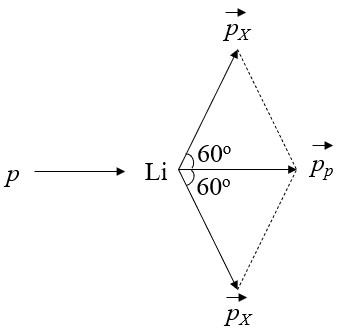
\includegraphics[scale=0.8]{../figs/VN12-PH-47-L-028-2-H1.jpg}
		\end{center}
		
		Phương trình phản ứng:
		\begin{equation*}
		^1_1 p + ^7_3\text{Li} \rightarrow 2 ^4_2 X
		\end{equation*}
		
		Áp dụng định luật toàn động lượng
		\begin{equation*}
		\vec{p}_p + \vec{0} = \vec{p}_X + \vec{p}_X
		\end{equation*}
		
		Do, hai hạt nhân $X$ giống nhau bay ra với cùng tốc độ theo các phương hợp với phương tới của proton các góc bằng nhau là $60^\circ$ nên
		\begin{eqnarray*}
		p_p^2 &=& p_X^2 + p_X^2 + 2 p_X p_X \cos 120^\circ\\
		\Rightarrow p_p &=& p_X\\
		\Rightarrow m_p v_p &=& m_X v_X\\
		\Rightarrow \dfrac{v_p}{v_X} &=& \dfrac{m_X}{m_p} \\
		\Rightarrow \dfrac{v_p}{v_X} &=& \dfrac{\SI{4}{u}}{\SI{1}{u}}\\
		\Rightarrow \dfrac{v_p}{v_X} &=& 4.
		\end{eqnarray*}
		
\begin{center}
	\textbf{Câu hỏi tương tự}
\end{center}				
Dùng một proton có động năng $ \SI{5,58}{MeV} $ bắn phá hạt nhân $ ^{23}_{11} \text{Na} $ đứng yên sinh ra hạt $ \alpha $, hạt nhân $ X $ và không kèm bức xạ $ \gamma $. Biết năng lượng tỏa ra trong phản ứng chuyển hết thành động năng của các hạt tạo thành, động năng của hạt $ \alpha $ là $ \SI{6,6}{MeV} $	và động năng của hạt $ X $ là $ \SI{2,648}{MeV} $. Cho khối lượng các hạt tính theo $ u $ bằng số khối. Góc tạo bởi hướng chuyển động của hạt proton là
\begin{mcq}(4)
	\item $ 147^\circ $.
	\item $ 148^\circ $.
	\item $ 150^\circ $.
	\item $ 120^\circ $.
\end{mcq}

\textbf{Đáp án:} C.}
		
		\viduii{4}
		{
		[THPT QG 2019 - Mã đề 202] Dùng hạt $\alpha$  có động năng K bắn vào hạt nhân  $^{14}_{\ 7}\text{N}$ đứng yên gây ra phản ứng: $^4_2\text{He} + ^{14}_{\ 7}\text{N}\ \rightarrow X + ^1_1\text{H}$. Phản ứng này thu năng lượng $\SI{1,21}{\mega\electronvolt}$ và không kèm theo bức xạ gamma. Lấy khối lượng các hạt nhân tính theo đơn vị $u$ bằng số khối của chúng. Hạt nhân $X$ và hạt nhân $^1_1\text{H}$  bay ra theo các hướng hợp với hướng chuyển động của hạt $\alpha$  các góc lần lượt là $23^\circ$ và $67^\circ$ . Động năng của hạt nhân $X$ là
		
		\begin{mcq}(2)
			\item $\SI{0,775}{\mega\electronvolt}$.
			\item $\SI{3,89}{\mega\electronvolt}$.
			\item $\SI{1,27}{\mega\electronvolt}$.
			\item $\SI{1,75}{\mega\electronvolt}$.
		\end{mcq}}
		{
		\begin{center}
			\textbf{Hướng dẫn giải}
		\end{center}
		
		\begin{center}
			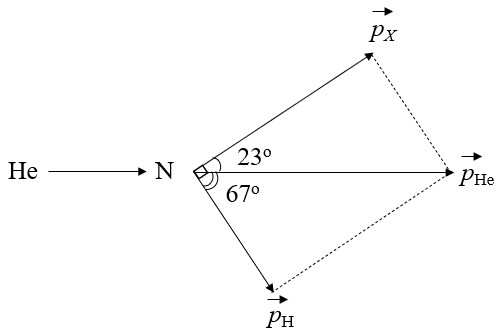
\includegraphics[scale=0.8]{../figs/VN12-PH-47-L-028-2-H2.jpg}
		\end{center}
	
		Phương trình phản ứng
		\begin{equation*}
		^4_2\text{He} + ^{14}_{\ 7}\text{N}\ \rightarrow ^{14}_{\ 8} X + ^1_1\text{H}.
		\end{equation*}
		 
		 Áp dụng định luật bảo toàn động lượng
		 \begin{equation*}
		 \vec{p}_X=\vec{p}_\text{He}+\vec{p}_\text{H}.
		 \end{equation*}
		 
		 Áp dụng định lý hàm sin
		 \begin{equation*}
		 \dfrac{p_\text{He}}{\sin 90^\circ}=\dfrac{p_\text{H}}{\sin 23^\circ}=\dfrac{p_X}{\sin 67^\circ}
		 \end{equation*}
		 \begin{equation*}
		 \Rightarrow
		 \left\{\begin{array}{ll}{p_\text{He}=\dfrac{\sin 90^\circ}{\sin 67^\circ}{p_X}}&\\
		 {p_\text{H}=\dfrac{\sin 23^\circ}{\sin 67^\circ}{p_X}}&\end{array}\right.
		 \end{equation*}
		 \begin{equation*}
		 \Rightarrow\left\{\begin{array}{ll}{p_\text{He}=1,086p_X}&\\{p_\text{H}^{2}=0,424p_X}&\end{array}\right.
		 \end{equation*}
		 \begin{equation*}
		 \Rightarrow\left\{\begin{array}{ll}{p_\text{He}^{2}=1,18p_X^2}&\\{p_\text{H}^{2}=0,18p_X^2}&\end{array}\right.
		 \end{equation*}
	 	\begin{equation*}
	 	\Rightarrow \left\{\begin{array}{ll}{2{m_\text{He}}{W_\textrm{đ He}}=1,18\cdot2{m_X}{W_\textrm{đ X}}}&\\
	 	{2{m_\text{H}}{W_\textrm{đ H}}=0,18\cdot2{m_X}{W_\textrm{đ X}}}&\end{array}\right.
	 	\end{equation*}
		\begin{equation*}
		 \Rightarrow \left\{\begin{array}{ll}{{W_\textrm{đ He}}=5,015W_{\textrm{đ }X}}&\\
		 {{W_\textrm{đ H}}=3,06W_{\textrm{đ }X}}.&\end{array}\right.
		 \end{equation*}
		 
		 
		 Áp dụng định luật bảo toàn năng lượng
		 \begin{equation*}
		 W_\textrm{đ He} - \SI{1,21}{\mega\electronvolt}= W_{\textrm{đ }X} + W_\textrm{đ H}
		 \end{equation*}
		 \begin{equation*}
		 \Rightarrow 5,015W_{\textrm{đ }X} - \SI{1,21}{\mega\electronvolt} = W_{\textrm{đ }X} + 3,06W_{\textrm{đ }X}
		\end{equation*}
		\begin{equation*}
		\Rightarrow W_{\textrm{đ }X}=\SI{1,27}{\mega\electronvolt}.
		\end{equation*}

\begin{center}
	\textbf{Câu hỏi tương tự}
\end{center}
Bắn phá một proton vào hạt nhân $ ^{7}_{3} \text{Li} $ đang đứng yên. Phản ứng hạt nhân sinh ra hai hạt nhân $ X $ giống nhau và có cùng tốc độ. Biết tốc độ của proton bằng $ 4 $ lần tốc độ của hạt nhân $ X $. Coi khối lượng của hạt nhân bằng số khối theo đơn vị $ u $. Góc tạo bởi phương chuyển động của hai hạt $ X $ là 
\begin{mcq}(4)
	\item $ 60^\circ $.	
	\item $ 90^\circ $.	
	\item $ 120^\circ $.	
	\item $ 150^\circ $.		
\end{mcq}

		\textbf{Đáp án:} C.
		}

	\end{dang}

